%------------------------------------------------------------------------------%
% Luis A. D'Afonseca
%
% T5
%------------------------------------------------------------------------------%
\documentclass[a4paper,12pt,fleqn]{article}

\usepackage{style_avaliacao}
\usepackage{graphicx}

\makeatletter
\graphicspath  {{./figs/}}
\def\input@path{{./figs/}}
\makeatother

\newcommand*{\prova}{Prova 1 -- Turma 5}
\newcommand*{\data}{31/08/2023}

%\usepackage{comment}
%\excludecomment{resposta}
\newenvironment{resposta}%
  {\begingroup\color{blue}\small\begin{spacing}{0.9}}%
  {\end{spacing}\endgroup}

%------------------------------------------------------------------------------%
\begin{document}

\makeHeader{Integrais e Séries}{\prova}{\data}

% 01
%------------------------------------------------------------------------------%
\exercise{25}
Dada a função
\(
  f(x) = \begin{cases}
    2 - x^2,                     & x \leq 1 \\[2mm]
    \hphantom{2}\frac{1}{\,x\,}, & x > 1    \\[1mm]
  \end{cases}
\)
\begin{enumerate}[label=\alph*)]
  \item Esboce o gráfico de $f$
  \item Calcule \( \int f(x)\,dx \)
  \item Calcule \( \int_0^e f(x)\,dx \)
\end{enumerate}

\begin{resposta}
\begin{enumerate}[label=\alph*)]
  \item Gráfico\\
    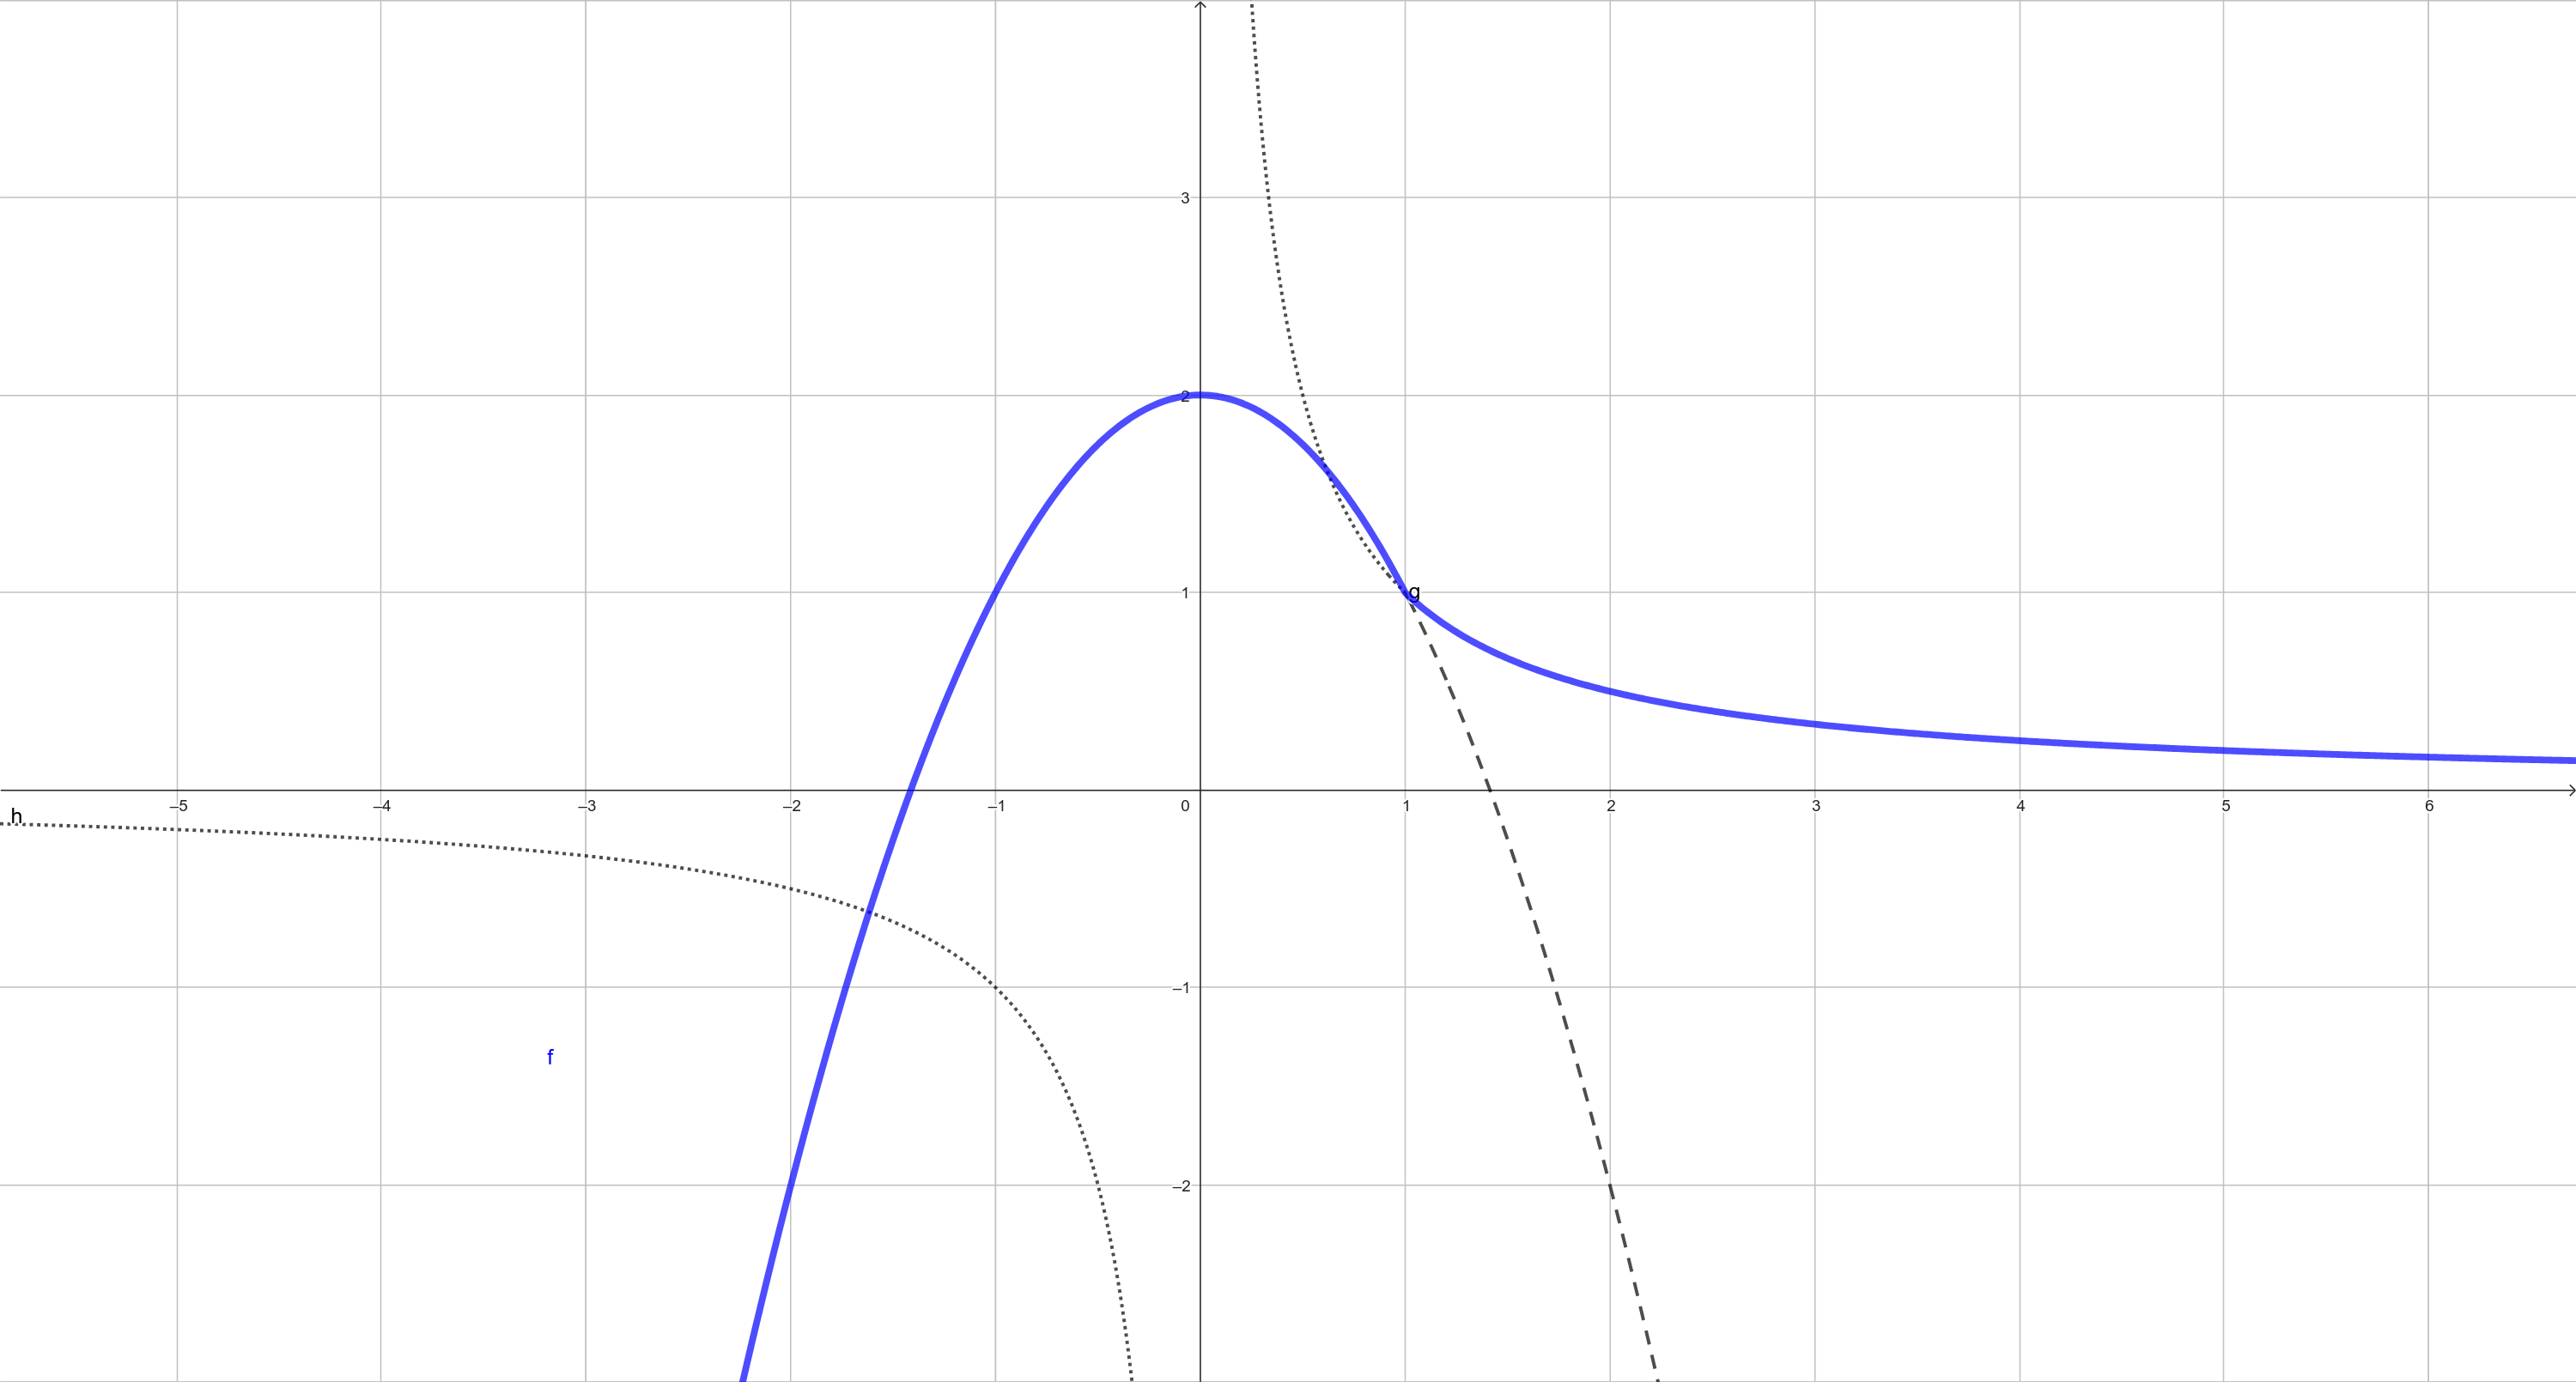
\includegraphics[height=6cm,width=\linewidth]{2_x2_1x}
  \item Considerando o intervalo $(-\infty, 1]$, temos
  \[
    \int f(x)\, dx
    = \int 2 - x^2\, dx
    = 2x - \frac{x^3}{3} + C_1
  \]
  No intervalo $(1, \infty)$, temos
  \[
    \int f(x)\, dx
    = \int \frac{1}{x}\, dx
    = \ln\abs{x} + C_2
    = \ln(x) + C_2
  \]
  Portanto a primitiva de $f$ é
  \[
    F(x) = \begin{cases}
      2x - \dfrac{x^3}{3} + C, & x < 0    \\[3mm]
      \ln(x) + C_2,           & x \geq 0
    \end{cases}
  \]

  \item Para calcular a integral definida precisamos dividir o intervalo em duas partes
  \begin{align*}
  I
  & = \int_0^e f(x)\,dx                         \\
  & = \int_0^1 f(x)\,dx + \int_0^\pi f(x)\,dx     \\
  & = \int_0^e 2-x^2\,dx + \int_1^e \frac{1}{x}\,dx \\
  & = \left(2x - \dfrac{x^3}{3}\right) \evalat{0}{1}
    + \ln(x) \evalat{1}{e}                          \\
  & = \left(2-\frac{1}{3}\right) - 0 + \ln(e) - \ln(1) \\
  & = 2-\frac{1}{3} + 1 \\
  & = \frac{8}{3}
  \end{align*}
\end{enumerate}
\end{resposta}

% 02
%------------------------------------------------------------------------------%
\exercise{25}
Data a função \(f(x) = \frac{1}{\sqrt{x^3}}\)
\begin{enumerate}[label=\alph*)]
  \item Esboce o gráfico de $f$
  \item Calcule sua primitiva
  \item Calcule \( \int_1^\infty f(x)\,dx \)
\end{enumerate}

\begin{resposta}
\begin{enumerate}[label=\alph*)]
  \item Gráfico\\
    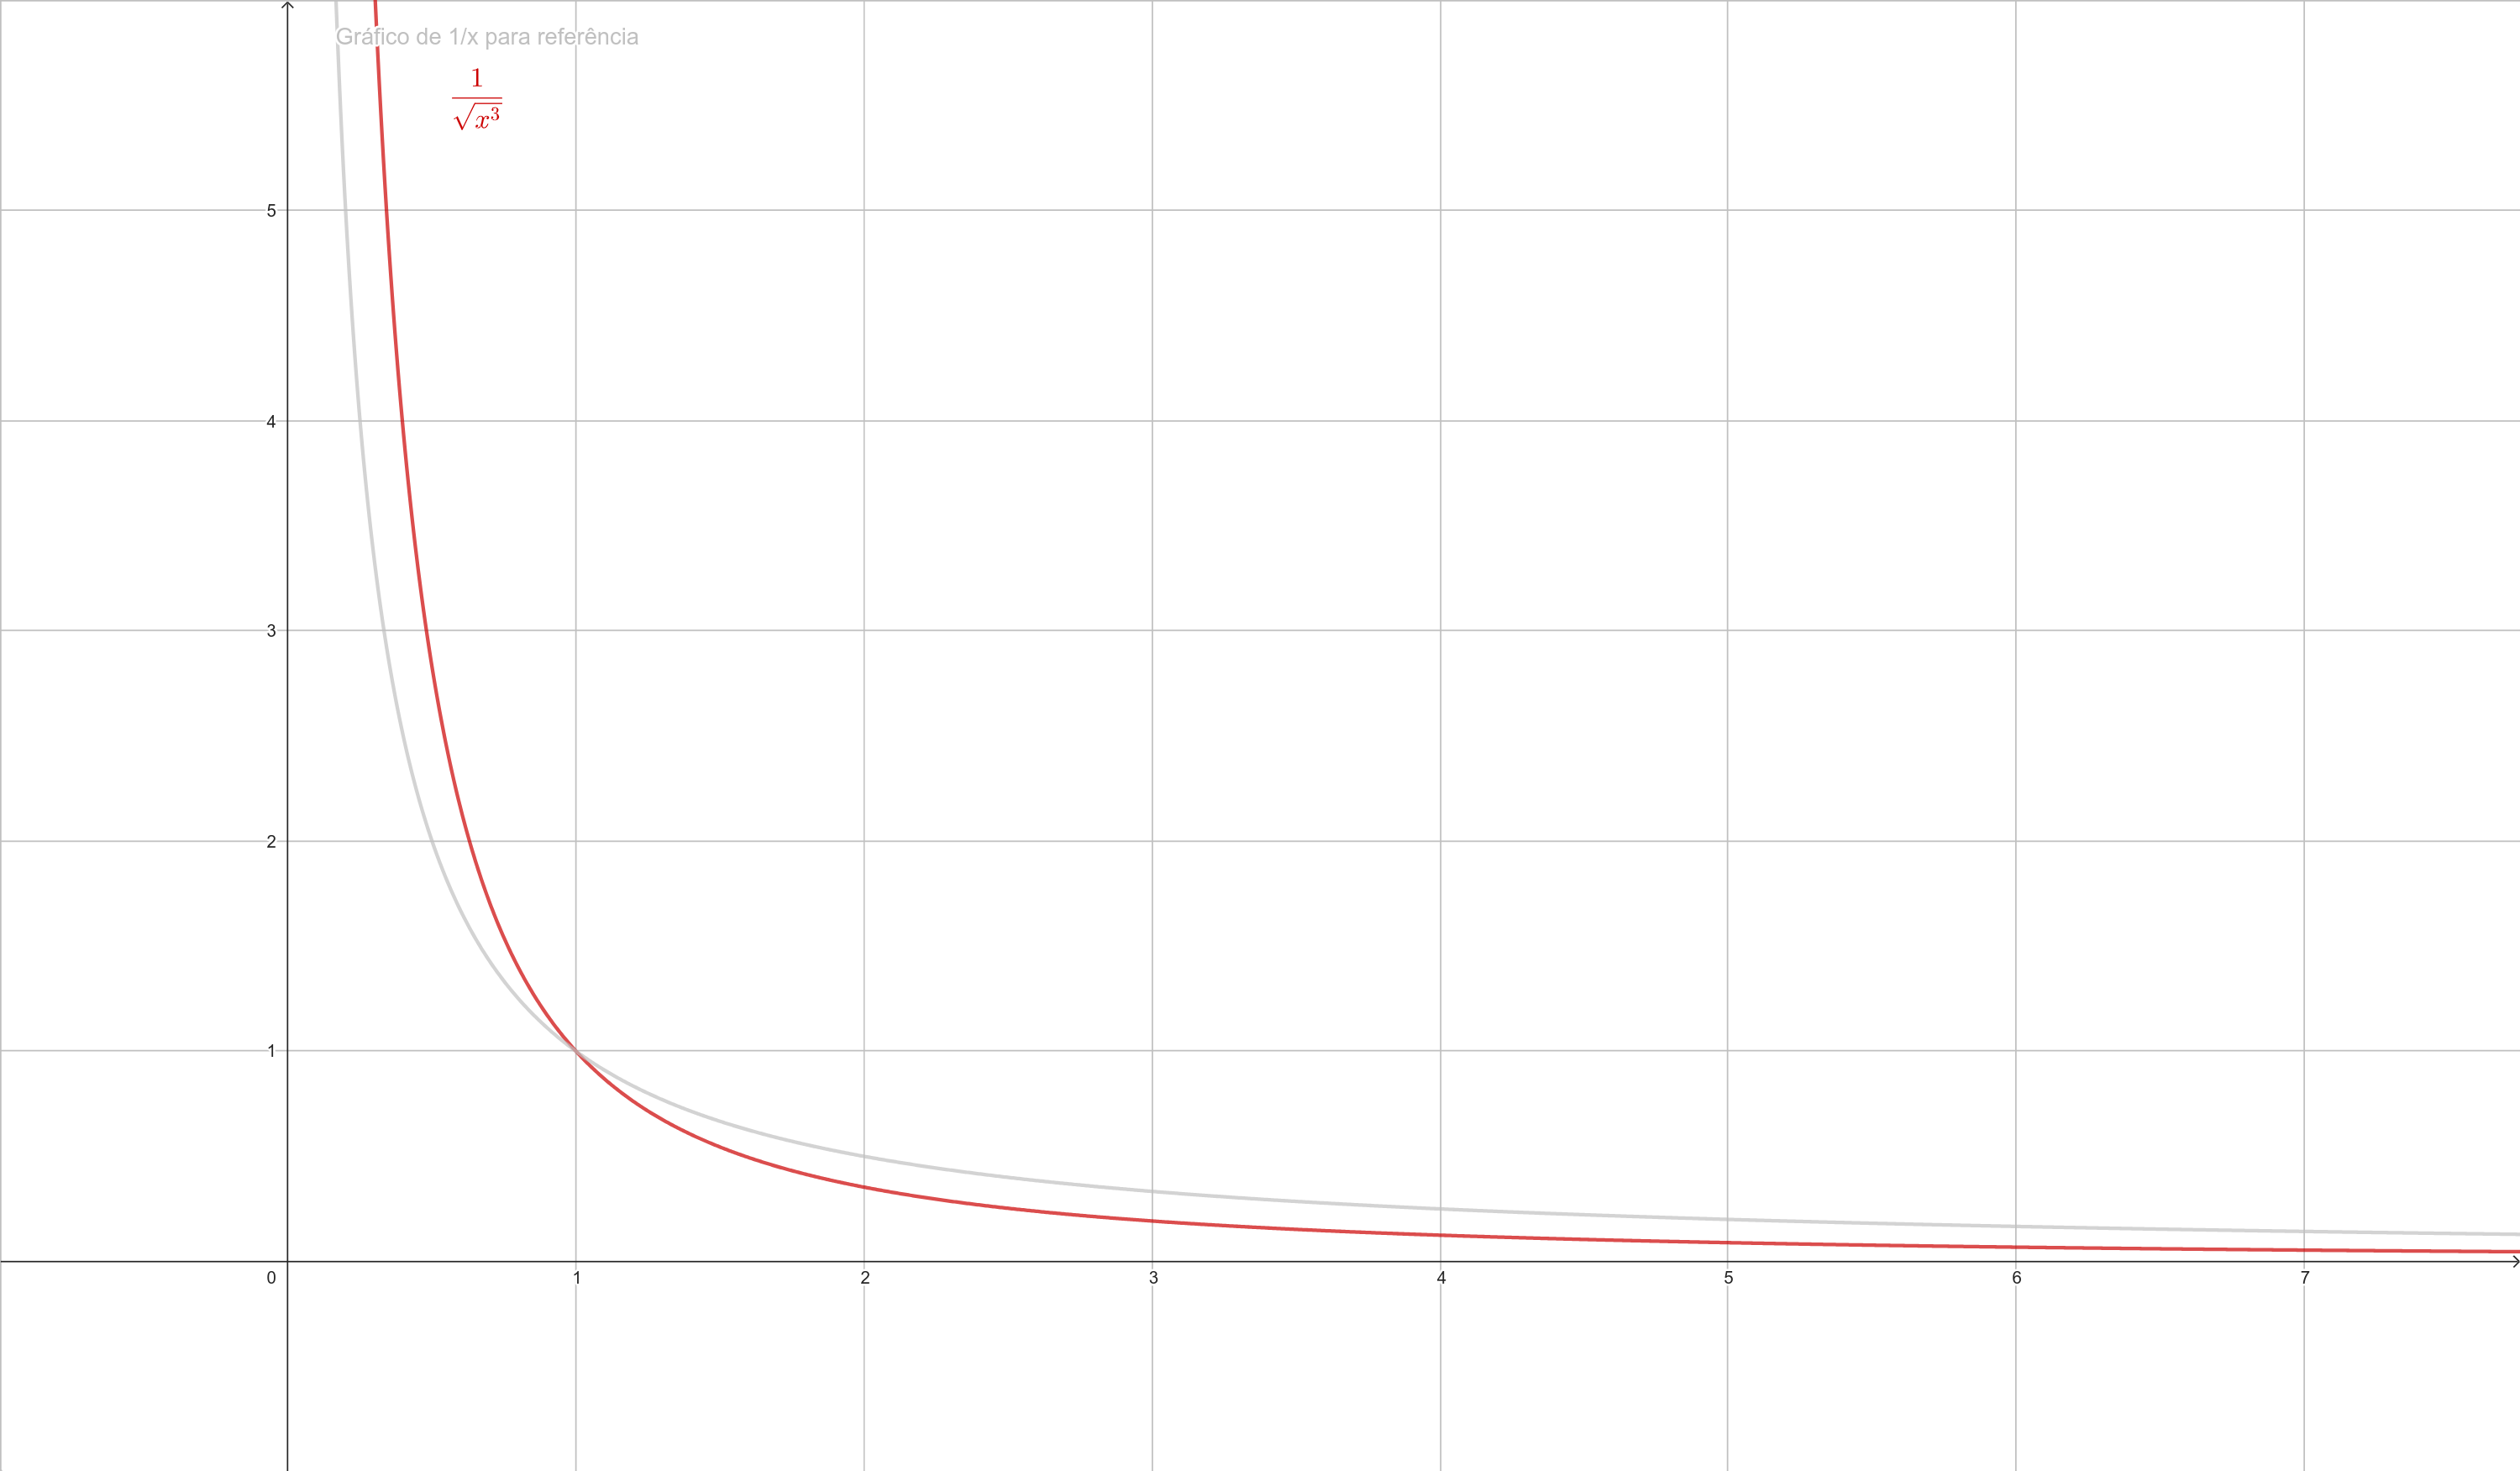
\includegraphics[height=6cm,width=\linewidth]{1_sqrt_x_3}
  \item
    \(
      \int f(x) dx
      = \int \frac{dx}{\sqrt{x^3}}
      = \int \frac{dx}{x^{\sfrac{3}{2}}}
      = \int x^{-\sfrac{3}{2}} dx
      = \frac{x^{-\sfrac{3}{2}+1}}{-\sfrac{3}{2}+1} + C
      = \frac{x^{-\sfrac{1}{2}}}{-\sfrac{1}{2}} + C
      = \frac{-2}{x^{\sfrac{1}{2}}} + C
      = \frac{-2}{\sqrt{x}} + C
    \)
    \item
    \(
    \int_1^\infty f(x) dx
      = \lim_{b\to\infty} \int_1^b x^{-\sfrac{3}{2}} dx
      = \lim_{b\to\infty} \left(\frac{-2}{\sqrt{x}}\right)\evalat{1}{b}
      = \lim_{b\to\infty} \left[\frac{-2}{\sqrt{b}} - \left(\frac{-2}{\sqrt{1}}\right)\right]
      = \lim_{b\to\infty} \frac{2}{\sqrt{a}} + 2
      = 2
    \)
\end{enumerate}
\end{resposta}

% 03
%------------------------------------------------------------------------------%
\exercise{25}
Considerando as curvas
\[
  y = \sin(x),
  \qquad
  y = x,
  \qquad
  x = \frac{\pi}{2}
  \qquad\text{e}\qquad
  x = \pi
\]
\begin{enumerate}[label=\alph*)]
  \item Esboce o gráfico das curvas e indique a área entre elas
  \item Calcule a área
\end{enumerate}

\begin{resposta}
  \begin{enumerate}[label=\alph*)]
    \item Gráfico\\
      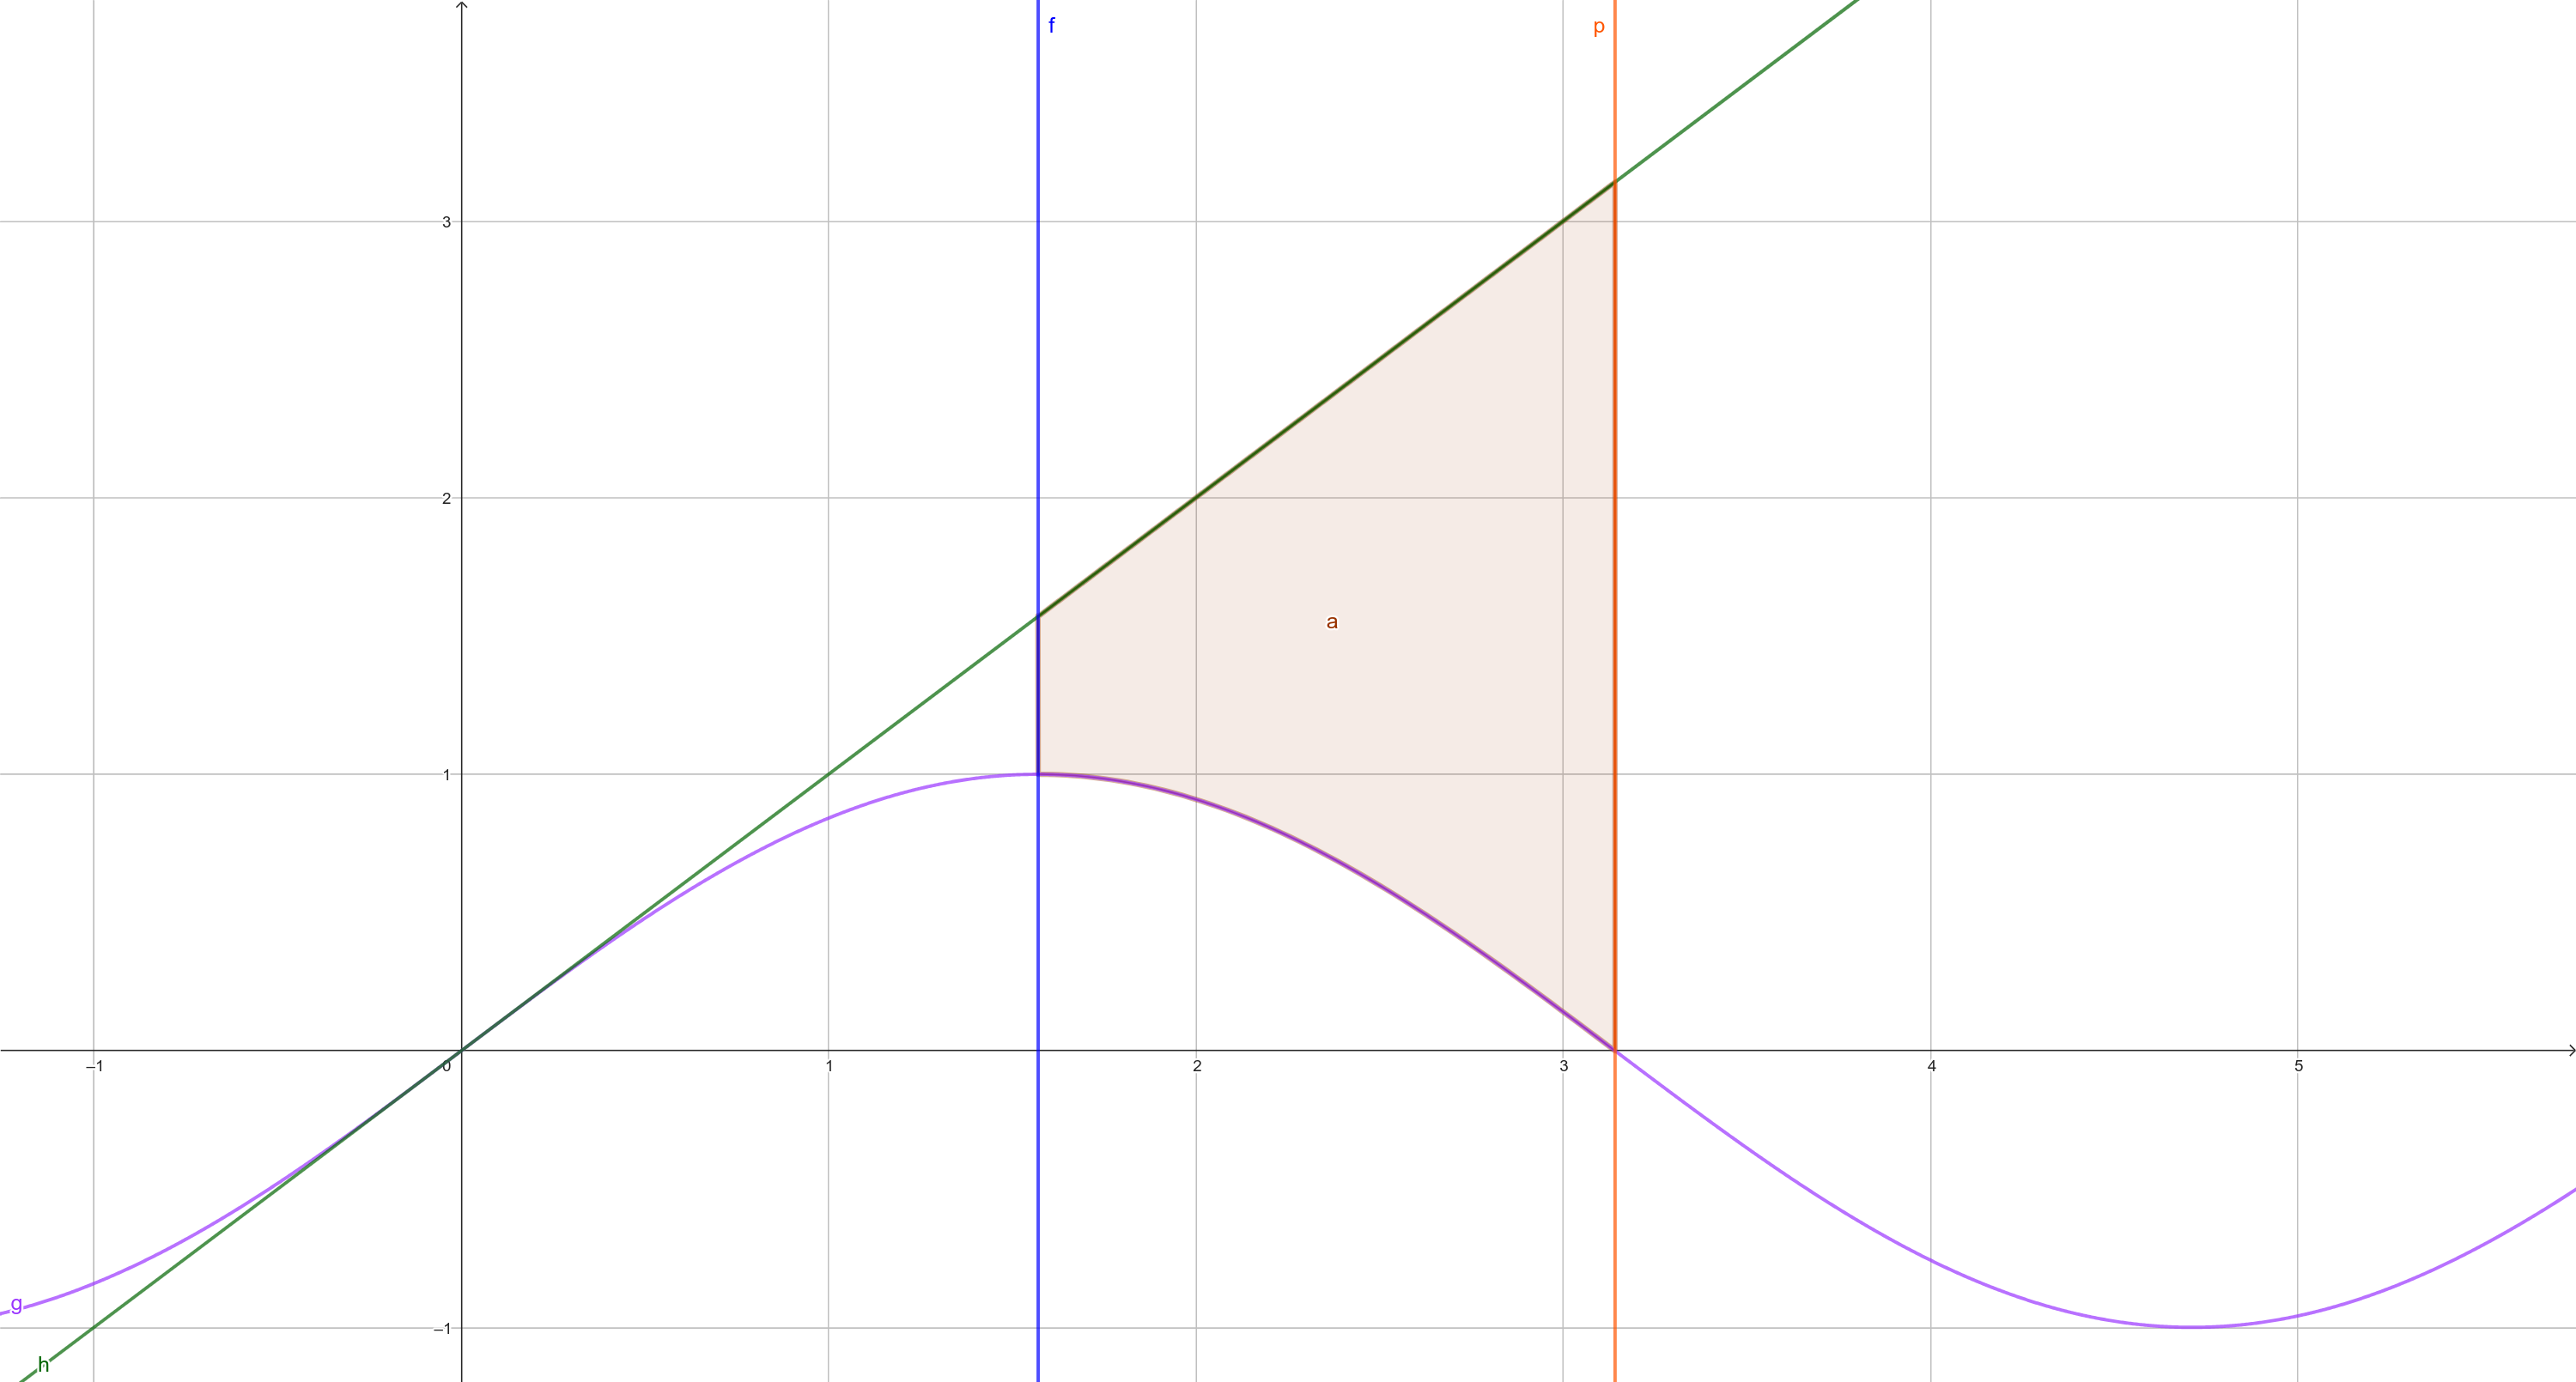
\includegraphics[height=6cm,width=\linewidth]{area_T5}
    \item
    \begin{align*}
      A & = \int_{\sfrac{\pi}{2}}^\pi x - \sin(x) \,dx \\
        & = \left( \frac{x^2}{2} + \cos(x)\right) \evalat{\sfrac{\pi}{2}}{\pi} \\
        & = \left( \frac{\pi^2}{2} + \cos(\pi)\right)
          - \left( \left(\frac{\pi}{2}\right)^2\frac{1}{2}
                 + \cos\left(\frac{\pi}{2}\right)
            \right)\\
        & = \frac{\pi^2}{2}
          - \frac{\pi^2}{2\times 4}
          + \cos(\pi)
          - \cos\left(\frac{\pi}{2}\right)\\
        & = \frac{4\pi^2}{8} - \frac{\pi^2}{8} - 1 - 0
          = \frac{3}{8}\pi^2 - 1
    \end{align*}
  \end{enumerate}
\end{resposta}

% 04
%------------------------------------------------------------------------------%
\exercise{25}
Encontre o volume do sólido obtido pela rotação
da região limitada pelas curvas
\[
  y = x^2 + 1
  \qquad\text{e}\qquad
  y = 2
\]
em torno da reta
\(
 x = -1
\)

\begin{resposta}
  \vspace{\baselineskip}
  \noindent
  Calculando os pontos de interseção
  \begin{align*}
    x^2+1 & = 2     \\
    x^2   & = 1     \\
    x     & = \pm 1
  \end{align*}

  \noindent
  Esboçado o gráfico\\
  \centerline{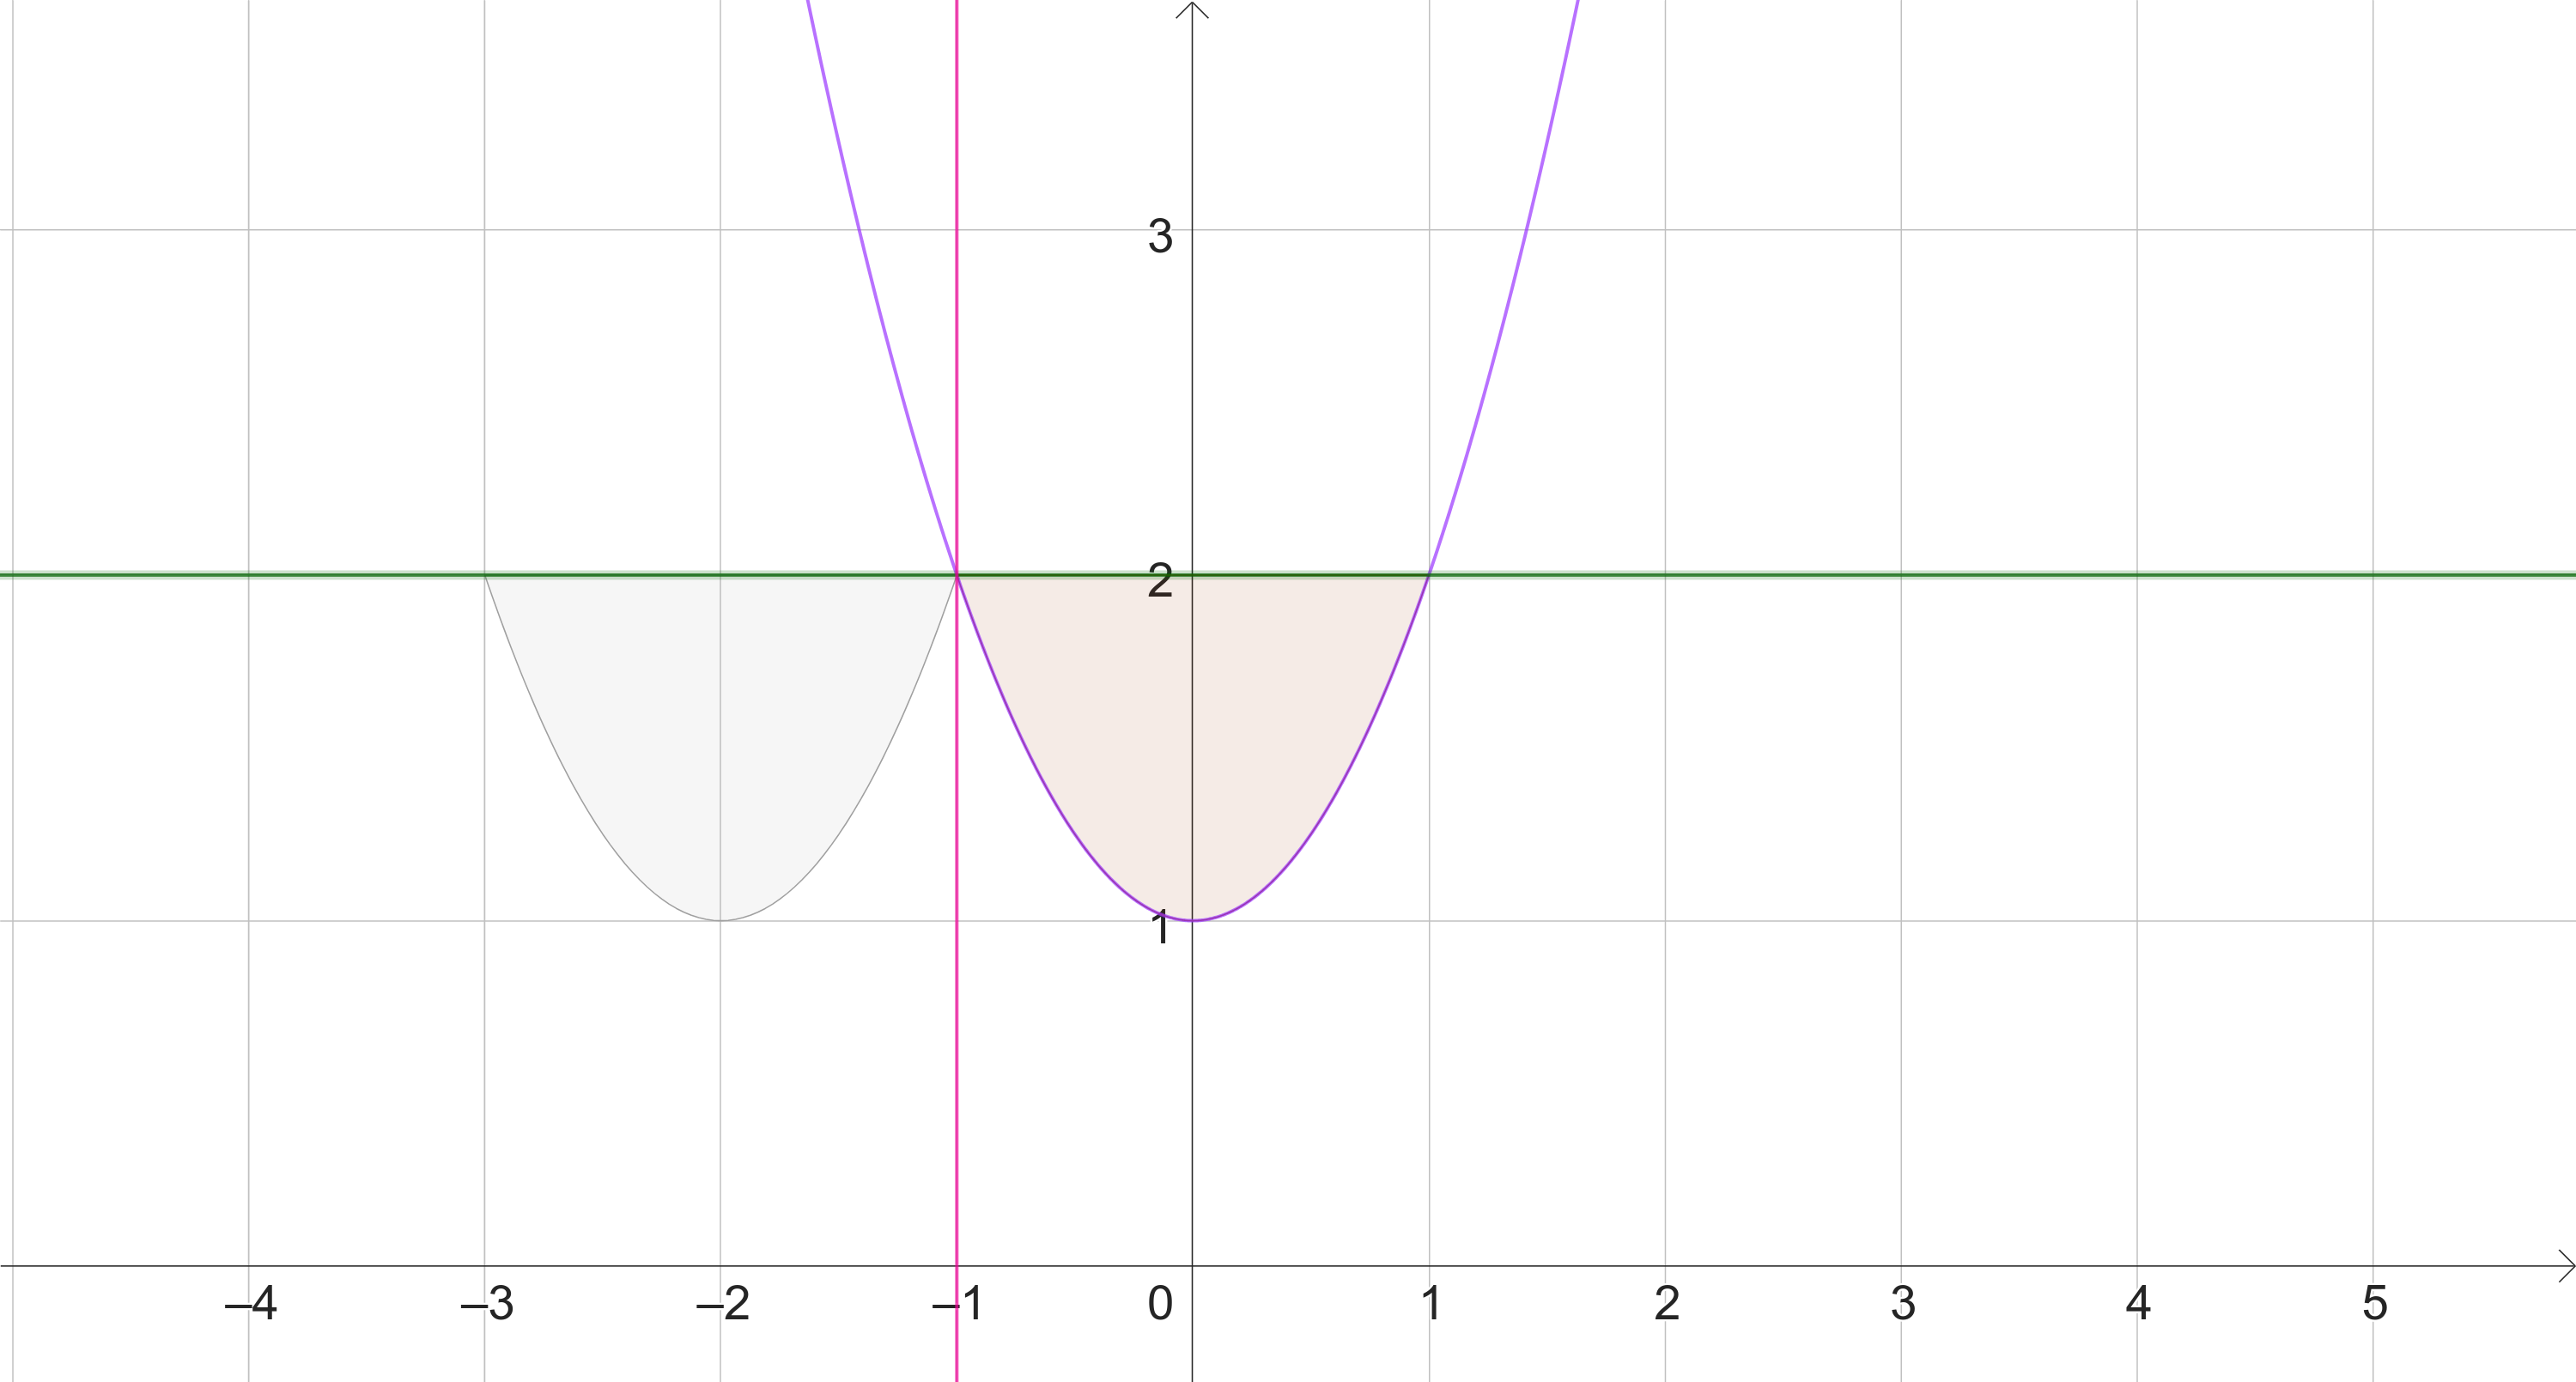
\includegraphics[height=6cm,width=\linewidth]{volume_T5}}

  \vspace{\baselineskip}
  \noindent
  Usando cascas cilíndricas, o volume é dado por
  \[
    V = \int_a^b 2\pi r(x) h(x) \,dx
  \]
  Pelo gráfico verificamos que
  \begin{align*}
    a & = -1 \\
    b & = 1 \\
    r(x) & = x + 1 \\
    h(x) & = 2-\left(x^2+1\right) = 1 - x^2
  \end{align*}
  Portanto
  \begin{align*}
    V
    & = \int_a^b 2\pi r(x) h(x) \,dx \\
    & = \int_{-1}^1 2\pi (x+1) \left(1-x^2\right) \,dx                  & \text{(15 pontos)}\\
    & = 2\pi \int_{-1}^1 x -x^3 + 1 - x^2\,dx \\
    & = 2\pi \int_{-1}^1 -x^3 - x^2 + x + 1 \,dx \\
    & = 2\pi \left(
            - \frac{x^4}{4}
            - \frac{x^3}{3}
            + \frac{x^2}{2}
            + x
            \right) \evalat{-1}{1} \\
    & = 2\pi \left[
      \left(
      - \frac{1^4}{4}
      - \frac{1^3}{3}
      + \frac{1^2}{2}
      + 1
      \right)
      - \left(
      - \frac{(-1)^4}{4}
      - \frac{(-1)^3}{3}
      + \frac{(-1)^2}{2}
      + (-1)
      \right)
      \right] \\
    & = 2\pi \left[
      - \frac{1}{4}
      - \frac{1}{3}
      + \frac{1}{2}
      + 1
      + \frac{(-1)^4}{4}
      + \frac{(-1)^3}{3}
      - \frac{(-1)^2}{2}
      - (-1)
      \right] \\
    & = 2\pi \left[
      - \frac{1}{4}
      - \frac{1}{3}
      + \frac{1}{2}
      + 1
      + \frac{1}{4}
      - \frac{1}{3}
      - \frac{1}{2}
      + 1
      \right] \\
    & = 2\pi \left[ 2 - \frac{2}{3} \right] \\
    & = 2\pi \frac{4}{3}  \\
    & = \frac{8\pi}{3} & \text{(10 pontos)}
  \end{align*}
\end{resposta}

%------------------------------------------------------------------------------%
\end{document}
%------------------------------------------------------------------------------%
